\section{Implementierung}
Dieses Kapitel beschreibt die Umsetzung des Projekts im Detail. Es wird ein Überblick über den Implementierungsprozesse gegeben, der Vorgehensweise bei der Entwicklung und ein Einblick in Probleme, welche während der Entwicklung aufgetreten sind.
Neben einer schrittweisen Darstellung der Implementierung werden auch exemplarisch Codebeispiele vorgestellt.
\subsection[Implementierungsdetails]{Implementierungsdetails}
In den Implementieungsdetails werden die Vorgehensweisen und Konzepte, welche für die Implementierung des Fontends und Backends benötigt werden, erläutert.

\subsubsection[Frontend]{Frontend}
Das \gls{sapui5}-Framework verwendet zur Darstellung der Seiten sogenannte \textit{Views} welche in \gls{xml} Dateien definiert werden.
Diese Views müssen mit der Dateiendung "\textbf{.view.xml}"\ enden, damit sie von \gls{sapui5} als View erkannt werden.

Views sind eine Art Kontainer für \gls{sapui5}-Elemente (Buttons, Input Felder, Tabellen, Listen, ...) und \gls{sapui5}-Layouts (Flex Box, HBox, VBox).
Views können jedoch auch andere Views beinhalten und so einen verschachtelten Aufbau der Seite schaffen.
Die \gls{sapui5}-Elemente sind vorgefertigte Komponenten welche von \gls{sapui5} bereitgestellt werden, um eine einheitliche Benutzeroberfläche zu schaffen, welche dann auch über verschiedene SAP-Anwendungen in einem Unternehmen konsistent ist.

Für die Admin-UI Seite sollen die Views und Komponenten wie in Abbildung \ref{fig:appstructure} angeortnent und strukturiert werden.
Die Unterseiten für die Eingabefelder aus den Anforderungen \ref{Tab:A4}, \ref{Tab:A5} und \ref{Tab:A6} werden in eigenen Views angezeigt, zwischen denen der Benutzer über die Navigationsleiste wechseln kann.

\begin{figure}[H]
    \centering
    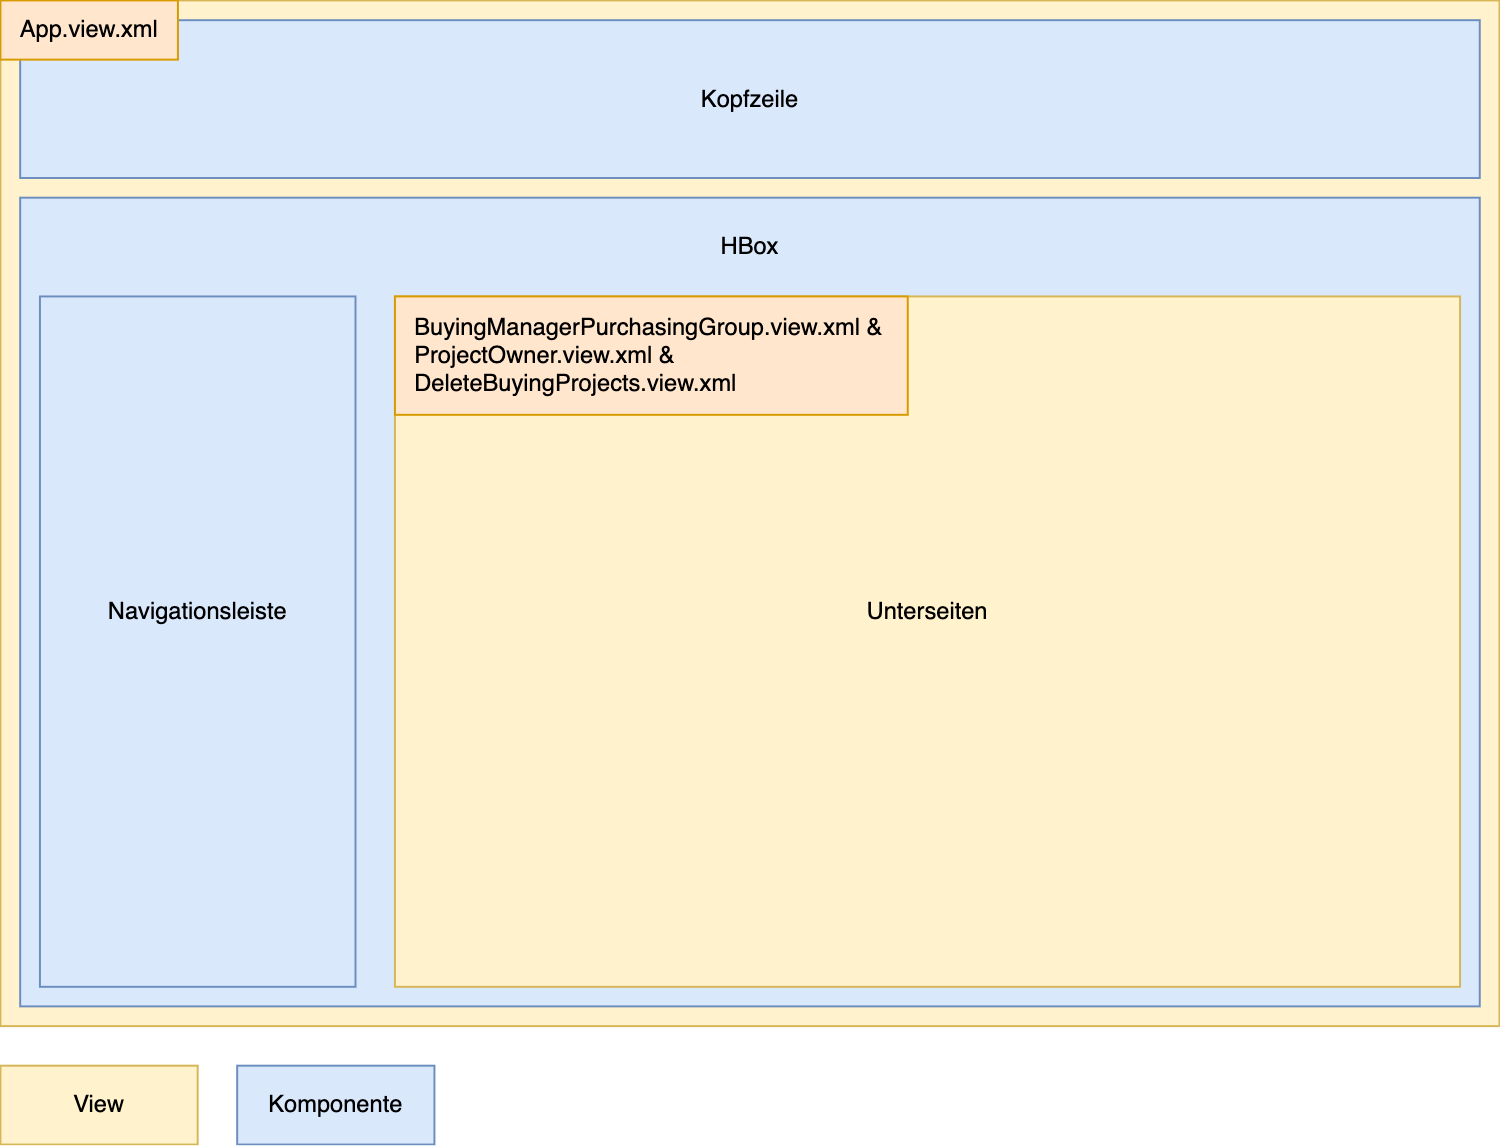
\includegraphics[width=\linewidth]{Images/AppStructure.png}
    \caption[Darstellung der Anwendungsstruktur]{Darstellung der Anwendungsstruktur}
    \label{fig:appstructure}
\end{figure}

Für jeden View kann ein \textit{Controller} erstellt werden, welcher die Funktionalität für die Views bereitstellt und Elemente dynamisch laden kann. 
Ein muss, so wie die View, eine besondere Dateiendung haben, damit \gls{sapui5} die Datei als Controller erkennen kann. Für Controller ist diese Endung "\textbf{.controller.ts}".

Für das Admin-UI soll für jeden View ein Controller erstellt werden. Zudem soll es einen sogenannten \textit{BaseContoller} geben, von dem alle anderen Controller seine Funktionen erben.
Dieser BaseController benötigt, anders also normale Controller, nicht die Controller spezifische Endung sondern nur die TypeScript spezifische Dateiendung "\textbf{.ts}".
Denn der BaseController wird keinem View explizit zugeordnet und muss daher auch nicht von \gls{sapui5} als Controller erkannt werden.  

Die Funktion eines BaseControllers ist es, Funktionen, welche von jedem Controller benötigt werden, in diesem zu definieren, damit diese an einer zentralen Stelle definiert sind und nicht in jedem Controller neu defniert werden müssen. 
Dazu gehören meist Helferfunktionen für zum Beispiel das Routing oder im Fall des Admin-UIs auch die Funktionalität der Aktionsleiste (siehe Anforderung \ref{Tab:A7}), welche auf jeder Unterseite eine sehr ähnliche Funktion hat.

In den Controllern für die einzelnen Unterseiten sollen Funktionen die spezifisch für die Unterseiten sind stehen, wie die intelligenten Vorschläge für die Eingabefelder (Anforderung \ref{Tab:A3}) und das Senden der Daten an das Backend.

\subsubsection[Backend]{Backend}
Im Backend sollen die Daten, welche von dem Frontend gesendet wurden, validiert und verarbeitet werden.

Für das Löschen einen Kaufprojekts muss jediglich die \textit{projectId} des zu löschenden Projektes gesendet werden, wofür eine \gls{cap} \textit{function} verwendet werden soll.
Eine \gls{cap} \textit{function} kann Parameter haben und muss immer einen Rückgabewert haben und führt eine gewisse Aktion aus.

Für das Ändern der Projekt Owner und Manager, sowie der Purchasing Organisation, soll für jede Änderung ein neuer Eintag in eine Datenbanktabelle geschrieben werden, der die alten und neuen Werte, sowie den Benutzer der die Änderung getätigt hat und den Zeitpunkt der Änderung beinhaltet.
Diese Datenbanktabellen sind in Abbildung \ref{fig:masschangetables} dargestellt.
Dies soll dazu dienen, die Änderungen auch im Nachhinein nachvollziehen zu können oder auch Rückgeängig zu machen. 

\begin{figure}[H]
    \centering
    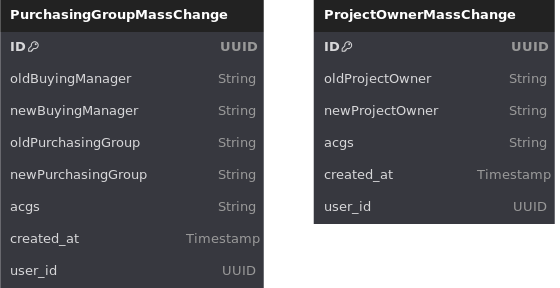
\includegraphics[width=.6\linewidth]{Images/MassChangeTables.png}
    \caption[Datenbanktabellen für Massenänderungen]{Datenbanktabellen für Massenänderungen}
    \label{fig:masschangetables}
\end{figure}

Wenn aus dem Frontend ein neuer Eintrag in einer der Tabelle erstellt wird, soll mit einer sogenannten \textit{Hook} in \gls{cap} das Änderen der Daten geschehen.
Diese \textit{Hooks} fangen das Erstellen der Tabelle ab und führen dann individuellen Code aus, in dem die gesendeten Daten verarbeitet werden können.

Bevor jedoch die Daten verarbeitet werden, muss überprüft werden, ob der Benutzer, der die Daten gesendet hat, die Berechtigung hat diese Änderungen durchzuführen.
Falls dies nicht der Fall ist, soll ein Error an das Frontend gesendet werden und eine entsprechende Errornachricht angezeigt werden.
Wenn der Benutzer jedoch die benötigte Berechtigung besitzt sollen die Daten verarbeitet und validiert werden und die Änderungen in der Datenbank vorgenommen werden.

\subsection[Schrittweise Beschreibung der Implementierung]{Schrittweise Beschreibung der Implementierung}

In diesem Abschnitt werden die Implementierungsdetails aus dem vorherigen Abschnitt anhand von Codebeispielen schrittweise erläutert und erklärt.

\subsubsection{Frontend}
Die Implementierung des Frontends teilt sich in zwei Abschnitte auf. 
Zum einen die Erstellung der Views, welche die Darstellung der Seite seien werden, und die Erstellung der Controller, zum anderen die Views mit Funktionalität zu versehen. 

\textbf{Erstellung der XML-Views:}

Für die Darstellung wurden, wie in Abbildung \ref{fig:appstructure} bereits dargestellt wurde, vier verschiende \gls{xml}-Views angelegt.
Die \textit{App.view.xml}, \textit{BuyingManagerPurchasingGroup.view.xml}, \textit{ProjectOwner.view.xml} und die \textit{DeleteBuyingProjects.view.xml}.

Für die App-View wurden drei Hauptkomponenten benötigt.
Die Kopfzeile mit dem Titel der Seite, die Navigationsleiste zur Navigation zwischen den Unterseiten und die Unterseiten an sich, welche dynamisch mit Hilfe der Naviagtionsleiste angezeigt werden.
All diese Komponenten wurden innerhalb einer \textit{DynamicPage-Komponente} definiert, welche bereits Funktionalitäten für eine einfahrbare Kopfzeile und Navigationsleiste bietet.
So konnte die Kopfzeile als eine \textit{DynamicPageTitle und DynamicPageHeader-Komponente} als Titel und Header der DynamicPage hinzugefügt werden.
Wie das dann im Code für das Admin-UI aussieht, sehen Sie im folgenden Listing:

\begin{lstlisting}[caption={Kopfzeile des App-Views}, language={XML}]
<f:DynamicPage class="sapUiNoContentPadding">
    <f:title>
        <f:DynamicPageTitle>
            <f:heading>
                <Title text="{i18n>titHeader}" class="sapUiSmallMarginTop" />
            </f:heading>
        </f:DynamicPageTitle>
    </f:title>
    <f:header>
        <f:DynamicPageHeader>
            <VBox>
                <Label text="{i18n>lblVersion}" />
            </VBox>
        </f:DynamicPageHeader>
    </f:header>
    ...
</f:DynamicPage>
\end{lstlisting}

Das \textit{text}-Attribut, liefert den Text der in dem Titel und dem Header angezeigt werden.
Dieser kommt in unserem Fall aus dem \textit{i18n}-Model, welches Text in verschiedenen Sprachen bereitstellt.
Das \textit{class}-Attribut, ist für das Styling der Elemente verantwortlich. 
Hier wird eine von \gls{sapui5} vorgefertige Klasse angegeben, um ein einheitliches Aussehen auf der ganzen Seite zu garantieren.

Für die Navigationsleite und die Unterseiten wurden zwei \textit{Panel-Komponenten} verwendet, diese dienen als Kontainer für den Inhalt der Komponenten und haben die Möglichkeit sich ein- und ausklappen zu lassen.
Die Navigationsleite wurde als eine Liste von \textit{ActionListItems} definiert, welche eine Art Knöpfe sind, die durch Attribute als ausgewählt angezeigt werden können.
Diese \textit{ActionListItems} werden anhand von vordefinerten Routen dynamisch generiert und sind somit jeweils an eine Route, beziehungsweise an eine Unterseite gebunden.
Durch anklicken eines der \textit{ActionListItems} wird über den \gls{sapui5}-Router das richtige XML-View in den \textit{Panel-Kontainer} für die Unterseiten geladen.

In dem folgenden Listing wird der Code für die beiden \textit{Panel-Komponenten} dargestellt, es wurden jedoch Attribute und Elemente, welche jediglich für das Aussehen der Komonenten zuständig sich, ausgelassen. 

\begin{lstlisting}[caption={Navigationsleisten- und Unterseiten-Kontainer des Admin-UIs}, language={XML}]
...
<Panel>
    <List items="{routes>/routes}">
        <ActionListItem
            text="{
                parts: [
                    'routes>name'
                ], formatter: '.formatter.formatNavItemText'
            }"
            type="Navigation"
            navigated="{= ${routes>name} === ${routes>/currentRoute}}"
            press="onNavItemPress" />
    </List>
</Panel>
<Panel>
    <NavContainer id="navContainer" width="100%" height="100%" />
</Panel>
...
\end{lstlisting}

Die drei \gls{xml}-Views für die Unterseiten sind alle gleich aufgebaut und verwenden alle dieselben Komonenten zur Darstellung der \textit{Toolbar} zum Speichern der Änderungen und den Eingabefeldern.

Für die Toolbar wird die \textit{Toolbar-Komponente} von \gls{sapui5} verwendet und beinhaltet zwei Knöpfe.
Ein Knopf zum Speichern und ein Knopf, um alle Eingabefelder zu leeren. 
Im folgenden Listing wird der Code für die Toolbar, welche auf allen Seiten weitestgehend identisch ist, dargestellt:

\begin{lstlisting}[caption={Toolbar der Unterseiten}, label={lst:toolbar}, language={XML}]
<Toolbar id="toolbar" design="Solid">
    <ToolbarSpacer />
    <Button text="{i18n>btnSaveChanges}" type="Emphasized" press="onSaveChangesPress" />
    <Button text="{i18n>btnClear}" press="onClearPress" />
</Toolbar>
\end{lstlisting}

Die Eingabefelder wurden mit \textit{Input-Komponenten} umgesetzt, da diese bereits Funktionalitäten für intelligente Vorschläge, wie in Anforderung \ref{Tab:A3} beschreiben, besitzen.
Für eine bessere Formatierung wurde jedes Eingabefeld und dessen Titel, welcher als \textit{Label-Komponente} dargestellt wird, in einer \textit{VBox-Komponente} platziert.
In dem folgenden Listing wird der Code für das Eingabefeld beispielshaft an einem Eingabefeld auf der ProjectOwner.view.xml Unterseite dargestellt:

\begin{lstlisting}[caption={Eingabefeld für Unterseiten}, language={XML}]
<VBox width="100%">
    <Label text="{i18n>lblOldBuyingManager}" required="true" />
    <Input
        id="oldBuyingManagerInput"
        value="{form>/oldBuyingManager}"
        placeholder="{i18n>txtEmailPlaceholder1}"
        required="true"
        suggestionItems="{/AppUsers}"
        showSuggestion="true"
        suggest="onSuggest($event, 'user')"
        suggestionItemSelected="onSuggestionItemSelected">
        <core:Item key="{id}" text="{id}" />
    </Input>
</VBox>
\end{lstlisting}

Die Attribute \textit{suggest} und \textit{suggestionItemSelected} der Input-Komponente bekommen die Namen von Funktionen übergeben, welche in einem Controller für die Views definiert sind.
Die Funktion dieser Funktionen ist es die intelligenten Vorschläge anhand der Benutzereingabe anzuzeigen und beim Auswählen eines der Vorschläge diesen Wert für das Feld zu übernehmen.
Das Attribut \textit{required} ist dafür da anzuzeigen, ob das Eingabefeld ein Pflichfeld ist und es dieses auf \textit{true} gesetzt wird vor dem Speichern überprüft, ob in diesem Feld etwas eingegeben wurde.

\textbf{Erstellung der Controller:}
Eingie Funktionalitäten sind in allen Unterseiten identisch, daher wurde für diese Funktionen ein BaseController erstellt.
Funktionen in diesem Contoller, stehen allen Views zur Verfügung, wodurch der Code für diese Funktionalitäten nur ein mal geschreiben werden musste.

Andere Funktionalitäten sind jedoch spezifisch für eine Unterseite oder muss unterschiedlich implementiert werden, da es zum Beispielt unterschiedlich Eingabefelder auf den Seiten gibt.
Eine dieser Funktionen ist die \textit{onSaveChangesPress}-Funktion aus Listing \ref{lst:toolbar}, die für das Speichern der Eingabefelder zuständig ist.

In dieser Funktion wird jedes Eingabefeld kurz validiert, indem überprüft wird, ob all Pflichtfelder ausgefüllt sind.
Wenn dies der Fall ist, werden die eingegebenen Werte an, sowie der \gls{api}-Endpunkt, der auf dieser Unterseite aufgerufen werden soll, an eine Funktion in dem BaseController gesendet.

In folgendem Listing wird die onSaveChangesPress Funktion dargestellt:
\begin{lstlisting}[caption={onSaveChangesPress Funktion}]
onSaveChangesPress(event: Button$PressEvent): void {
    const formModel = this.getModel<JSONModel>("form"),
            isFormValid = this.validateInputFields(this.allInputIDs);

    if (!isFormValid) {
        event.getSource().setEnabled(false);
        return;
    }

    if (!formModel) {
        return;
    }

    const {
        oldProjectOwner,
        newProjectOwner,
        SCGs
    } = formModel.getData();

    this.createSaveChangesMessageBox(
        "/ProjectOwnerMassChange", 
        {                
            oldProjectOwner,
            newProjectOwner,
            acgs: SCGs
        },
        this.allInputIDs
    );
}
\end{lstlisting}

Die \textit{createSaveChangesMessageBox}-Funktion ist eine Funktion im BaseController, welche eine \textit{MessageBox-Komponente} erstellt, um den Nutzer um eine weitere Bestätigung zu fragen.
Bestätigt der Benutzer seine Entscheidung, wird in der \textit{createSaveChangesMessageBox}-Funktion die \textit{submitChanges}-Funktion aufgerufen.
Diese ist dafür verantwortlich die eingegebenen Daten an das Backend zu senden.
Um das zu tun wird in dem \gls{odata}-Model, welches mit dem Backend verbunden ist, ein neuer Eintrag erstellt.
Dafür benötigt es die Namen der Tabelle, sowie die Daten, die in die Tabelle geschrieben werden sollen.



\subsection[Herausforderungen und Problemlösungen]{Herausforderungen und Problemlösungen}

\subsection[Darstellung aufgetretener Herausforderungen]{Darstellung aufgetretener Herausforderungen}

\subsection[Beschreibung der Lösungsansätze]{Beschreibung der Lösungsansätze}
